\section{Electronics and Data Acquisition}
\label{sec:daq}
The SK Electronics and Data Acquisition System (DAQ) was extensively upgraded between SK-III and SK-IV.  As such, the SK-IV electronics will be explained separately from the SK I-III electronics.
\subsection{SK I-III}
\label{subsec:sk_1_3_daq}
The SK I-III DAQ processed ID PMT signals using custom build Analog-Timing-Modules (ATMs), which were originally designed and built by KEK.   A schematic of the ATM can be seen in \cref{fig:daq_ATM}  The PMT signal was split into four signals.  One of these signals was sent to a discriminator, which compared the signal to a threshold corresponding to 1/4 pe equivalent.  When the signal crossed this threshold, a 200ns wide logic pulse was sent to a hardware trigger module.  Simultaneously, the signal from the PMT was stored by a Charge-to-Analog Converter (QAC), and a integration of a constant current was started by a Time-to-Analog Converter (TAC).  When a global trigger was received from the hardware trigger module, the TAC integration was stopped and the information in the QAC and TAC were sent to and Analog-to-Digital Converter (ADC) to be digitized and stored in internal memory.  Because the TAC integrated a constant charge from the time of the channel trigger to the time of the global trigger, the time of the PMT signal relative to the global trigger can be calculated from the total integrated charge on the TAC.  Each channel was assigned two TACs and QACs, in order to process events which might occur in rapid succession, such as the a decay electron following a muon.  The charge dynamic range of the ATM was about 450 pC, with a resolution of 0.2 pC, while the timing dynamic range was 1.3 $\mu$s, with a resolution of 0.4 ns.\par
A hitsum was calculated by the hardware trigger module by simple analog sum of the logic signals from the ATMs.  When the hitsum crossed a given threshold, a global trigger would be issued to the ATMs.  Three different triggers were used: high energy (HE), low energy (LE) and super low energy (SLE).  The HE and LE triggers were set at 31 and 29 hits, respectively, with the LE threshold corresponding to an electron energy of 5.7 MeV.  The SLE trigger was added to lower the energy threshold to 4.6 MeV.  The trigger logic and interaction with the ATMs is shown in \cref{fig:daq_trigger_1_3}, and a full schematic of the DAQ is shown in         
\cref{fig:daq_schematic_1_3}.  The OD operated with a similar trigger system, and OD triggers were issued with a threshold of 19 hits.  Additional details of the ID and OD electronics and DAQ for SK I-III can be found in \cite{Fukuda:2002uc}. 
\begin{figure}
\centering
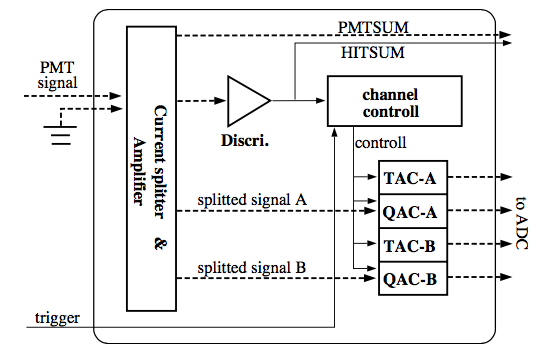
\includegraphics[width=0.5\textwidth]{figures/SK_1_3_ATM.png}
\caption{Schematic of processing of one channel by the ATM, used in SK I-III.  Dashed lines represent analog signals while solid lines represent logic signals \cite{Fukuda:2002uc}.}
\label{fig:daq_ATM}
\end{figure}

\begin{figure}
\centering
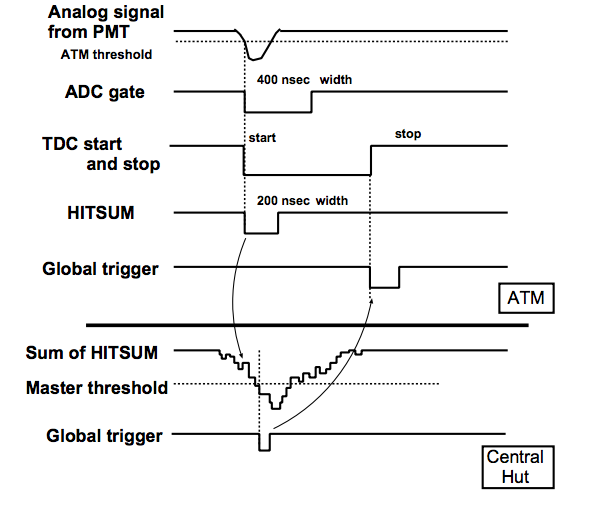
\includegraphics[width=0.5\textwidth]{figures/ID_trigger_SK1_3_Nishino.png}
\caption{Trigger system used in SK I-III \cite{Nishino:2009lps}.}
\label{fig:daq_trigger_1_3}
\end{figure}

\begin{figure}
\centering
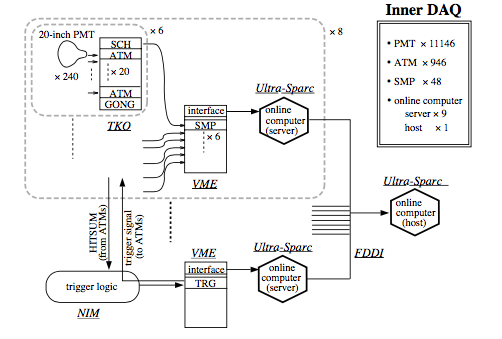
\includegraphics[width=0.5\textwidth]{figures/SK_1_3_daq.png}
\caption{Schematic of SK I-III DAQ.  Lines indicate flow of data \cite{Fukuda:2002uc}.}
\label{fig:daq_schematic_1_3}
\end{figure}

\subsection{SK-IV}
\label{subsec:sk_4_daq}
As mentioned earlier, the SK electronics were upgraded between SK-III and SK-IV \cite{Yamada:2010zzc,Nishino:2009zu}.  The ATM was replaced by a front end electronics board called a QBEE, which stands for "QTC (Charge-to-Time Converter) Based Electronics with Ethernet."   A QBEE is shown in \cref{fig:QBEE}.  PMT signals are processed by a QTC, which encodes the time and charge of the PMT pulse into the timing of a single pulse, as shown in \cref{fig:QTC_timing}.  When the PMT signal crosses a threshold which corresponds to about 1/4 pe (the same as in SK I-III), the QTC begins an output pulse, and a capacitor charges up over 400 ns with the charge from the PMT pulse.  The capacitor is then discharged at a constant rate, and the QTC output pulse is stopped when the capacitor charge drops below a comparator level.  The QTC output pulse thus encodes the time of the PMT pulse as the time of its leading edge, and the charge of the PMT pulse as its width. This full encoding and processing results in a deadtime of 900 ns.\par
Each PMT signal is processed by a QTC under three different gain settings, called ``Small", ``Medium" and ``Large", with gain ratios 1:$\frac{1}{7}$:$\frac{1}{49}$.  The charge dynamic ranges of the three gain setting are shown in \cref{tab:QTC_dynamic_ranges}.  While each PMT signal is process under all three gain settings, only the result from the lowest gain setting which is not saturated is used.  This results in a charge resolution similar to the ATMs used in SK I-III, but with about five times the dynamic range.\par   
The hardware trigger used in SK I-III is replaced by a software trigger for SK-IV.  Every hit recorded by the QBEEs is sent to Front-End PCs, with each Front-End PC receiving the hits from 30 QBEEs.  The data from the Front-End PCs is the sent on to Merger PCs, which combine the hits from all PMTs and apply software triggers to search for physics events.  When a software trigger is generated, the event data is sent to an Organizer PC, which writes the data onto disk for offline analysis.  This data flow is visualized in \cref{fig:sk_4_data_flow}.\par
The software trigger of SK-IV has multiple advantages over the hardware trigger of SK-III.  Primarily, it allows for any length of event, more complex trigger logic, and easy introduction of new triggers.  The main triggers used in SK-IV are summarized in \cref{tab:triggertable4}.  While the SLE, HE, SHE, and OD triggers perform functionality achievable which the SK I-III hardware trigger, the AFT trigger shows the true power of moving to a software trigger for SK-IV.  The AFT trigger is used for tagging neutrons, which capture and produce a 2.2 MeV $\gamma$ on the order of hundreds of $\mu$s after a primary neutrino event.  They do not produce enough hits to generate an SK I-III hitsum trigger, and lowering the hitsum threshold to catch such events would result in an significantly increased data rate and require substantially more computing power and disk space to handle.  This means that neutron tagging is impossible in SK I-III.  The software trigger of SK-IV solves all of these problems with the AFT trigger, which takes advantage of both the complex trigger logic and variable event width available in the software trigger system.    

\begin{table}
\centering
	\begin{tabular}{lcc}
	\hline \hline
	Gain Setting&Dynamic Range&Resolution\\
	\hline
	Low&51 pC&0.1 pC\\
	Medium&357 pC&0.7 pC\\
	High&2500 pC& 4.9 pC\\
   \hline \hline
	\end{tabular}
\caption{Charge dynamic ranges for the three gain settings of the SK-IV QTC.}
\label{tab:QTC_dynamic_ranges}
\end{table}

\begin{table}[!ht]
\centering
\begin{tabular}{lcccc}
\hline \hline
SK-IV Triggers & Trigger Logic & Event Width ($\mu s$) \\
\hline
SLE & 34 (31) hits in 200 ns & -0.5$\rightarrow$ 1.0 \\
HE & 50 hits in 200 ns & -5$\rightarrow$ 35 \\
SHE & 70 (58) hits in 200 ns & -5$\rightarrow$ 35\\
OD & 22 hits in 200 ns (in OD) & \\
AFT & SHE, no OD & 35 $\rightarrow$ 535 \\
\hline \hline
\end{tabular}
\caption{Trigger information for SK-IV. The abbreviations are as follows: 
OD (outer detector), SLE (super low energy), HE (high energy), SHE (
special high energy) and AFT (after).  The SLE and SHE trigger thresholds were lowered from 34 to 31 and 70 to 58 hits respectively, during SK-IV running.  There are $\sim$9 hits of dark noise 
in 200~ns and $\sim$6 hits corresponds to 1 MeV electron equivalent energy.}
\label{tab:triggertable4}
\end{table}

\begin{figure}
\centering
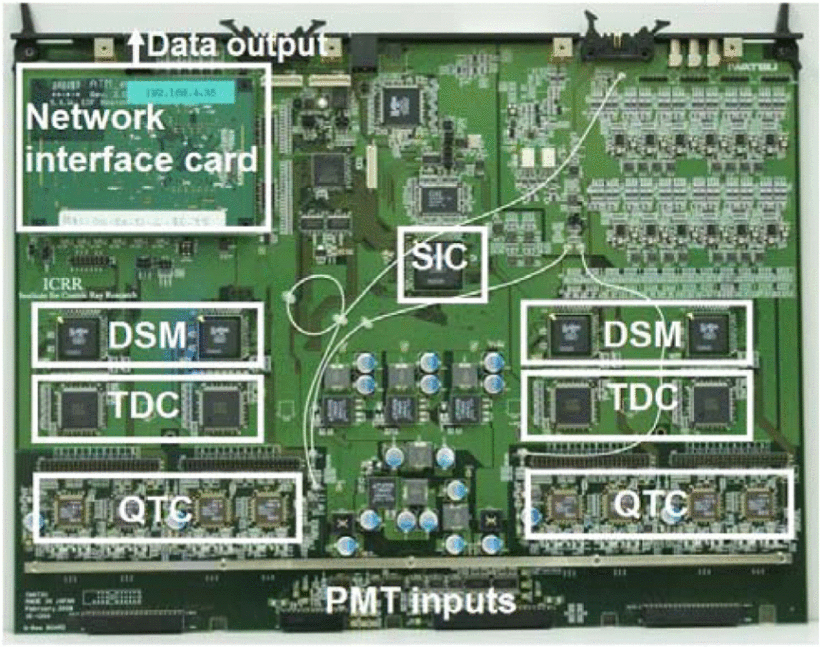
\includegraphics[width=0.5\textwidth]{figures/QBEE.png}
\caption{Front end electronics used in SK-IV, called QBEE \cite{Yamada:2010zzc}}
\label{fig:QBEE}
\end{figure}      

\begin{figure}
\centering
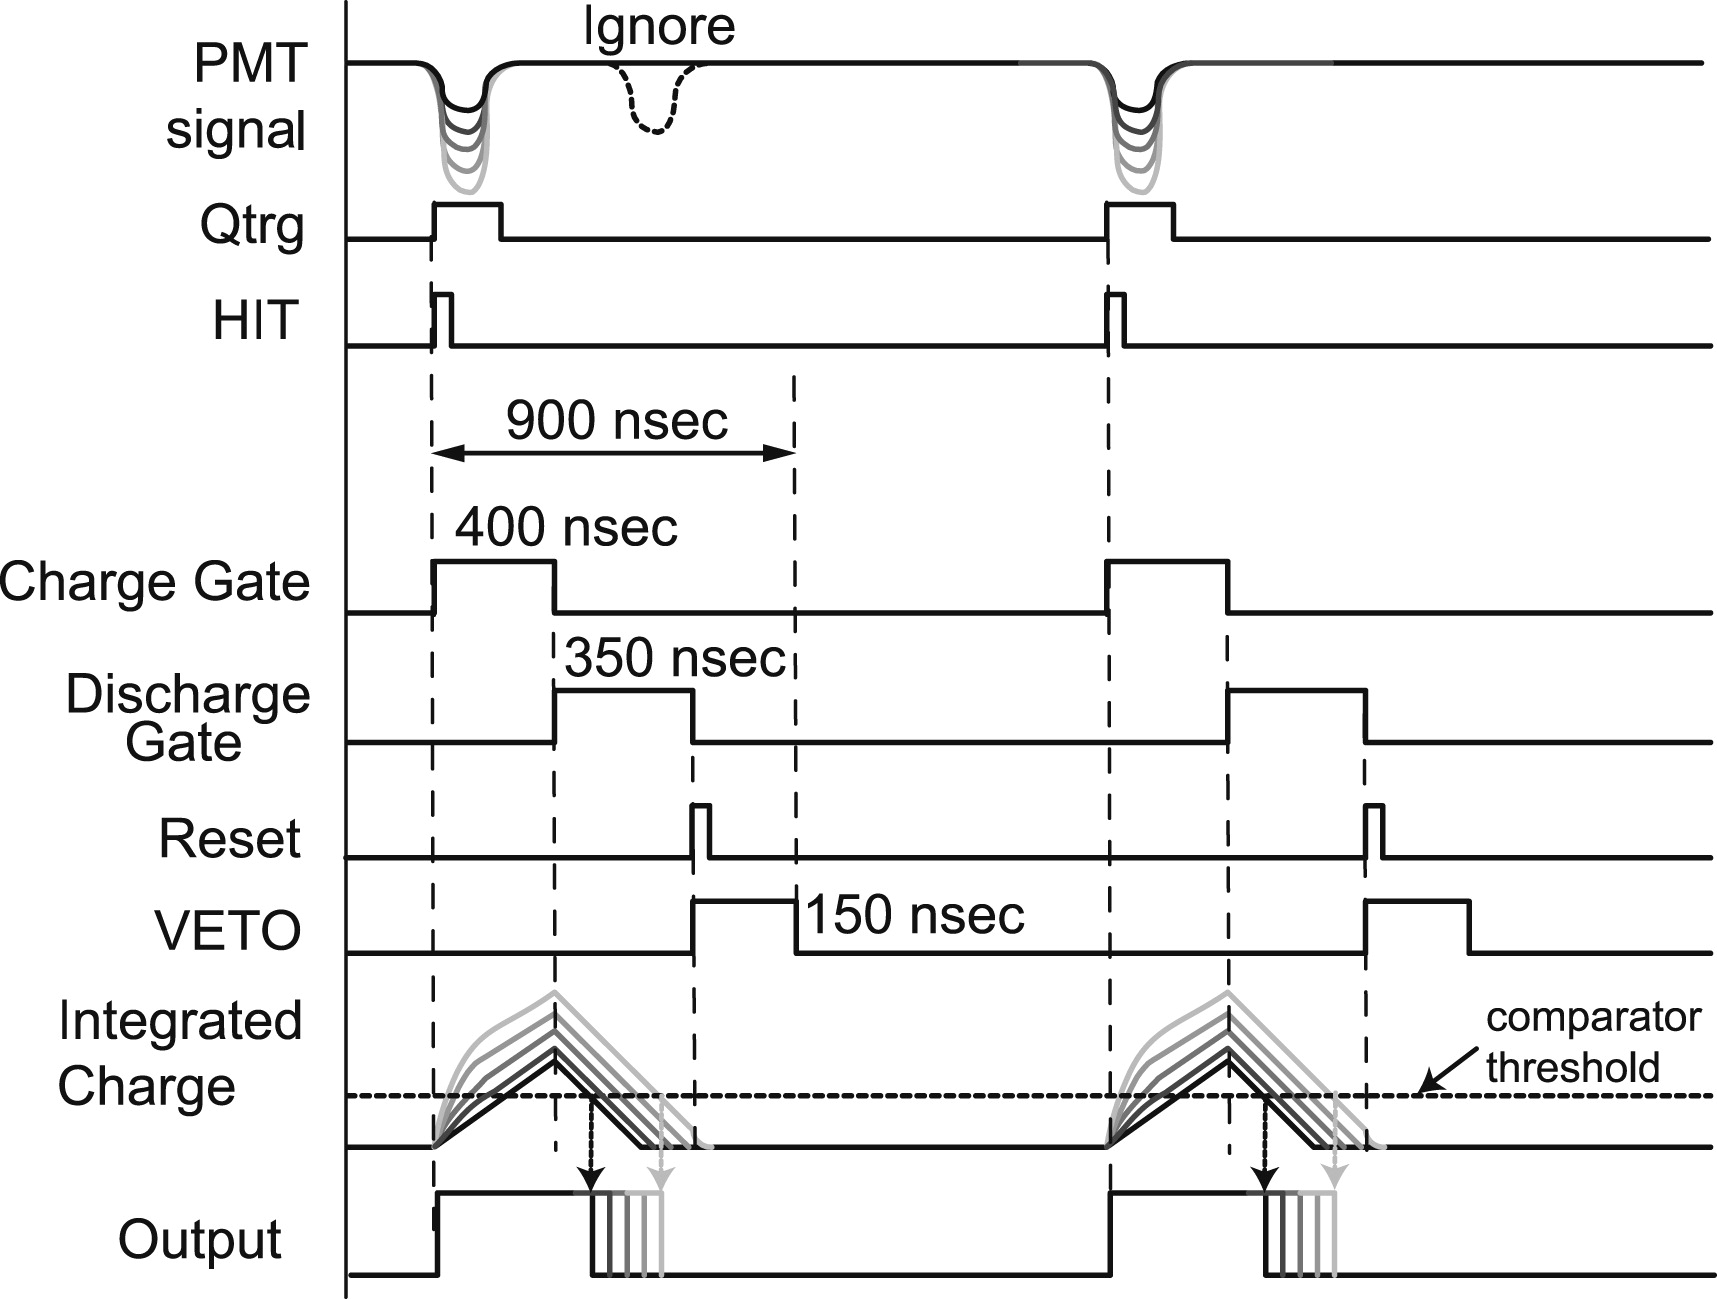
\includegraphics[width=0.5\textwidth]{figures/QTC_timing.jpg}
\caption{QTC charge and time encoding for QBEE \cite{Nishino:2009zu}.}
\label{fig:QTC_timing}
\end{figure}    

\begin{figure}
\centering
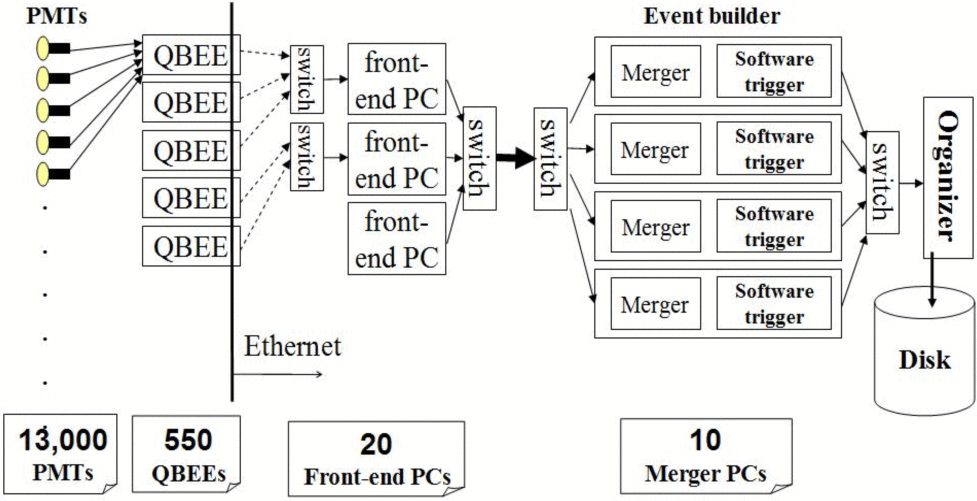
\includegraphics[width=0.5\textwidth]{figures/SK_4_data_flow.png}
\caption{SK-IV data flow \cite{Yamada:2010zzc}}
\label{fig:sk_4_data_flow}
\end{figure} 